\documentclass[11pt,letterpaper]{article}

% ============ EDITE AQUÍ SUS DATOS ANTES DE COMPILAR ============
\newcommand{\nombreEstudiante}{Duván Felipe Baquero}
\newcommand{\codigoEstudiante}{160005002}
\newcommand{\nombreDocente}{Ángel Alfonso Cruz Roa}
% ================================================================

% Codificación: compatible tanto con pdfLaTeX como con XeLaTeX/LuaLaTeX.
\usepackage{iftex}
\ifPDFTeX
  \usepackage[utf8]{inputenc}
  \usepackage[T1]{fontenc}
  \usepackage{lmodern}
\else
  \usepackage{fontspec}   % usa Latin Modern Unicode por defecto
\fi

% babel-spanish redefine \% e introduce su propio espaciado, lo que rompe
% construcciones como \,\% y el uso de \% dentro de modo matemático.
% Se guarda la versión original de LaTeX y se restaura tras cargar babel.
\let\origpercent\%
\usepackage[spanish,es-tabla]{babel}
\AtBeginDocument{\let\%\origpercent}
\usepackage[margin=2.5cm]{geometry}
\usepackage{graphicx}
\usepackage{booktabs}
\usepackage{longtable}
\usepackage{array}
\usepackage{makecell}
\usepackage{multirow}
\usepackage{amsmath}
\usepackage{amssymb}
\usepackage{float}
\usepackage{xcolor}
\usepackage{fancyhdr}
\usepackage{caption}
\usepackage{enumitem}
\usepackage{microtype}
\usepackage{tocloft}
\usepackage[hidelinks]{hyperref}

% Espacio vertical antes de cada entrada de sección (nivel 1) del índice.
% Se reduce un poco respecto al valor por defecto de article.cls (1.0em)
% para que "9. Anexos" quepa en la misma página que el resto del índice.
% Para volver al espaciado original, cambiar 0.7em de nuevo a 1.0em.
\setlength{\cftbeforesecskip}{0.7em}

\captionsetup{font=small,labelfont=bf,skip=6pt}
\setlength{\parskip}{0.35em}
\renewcommand{\arraystretch}{1.12}

\pagestyle{fancy}
\fancyhf{}
\lhead{\small Universidad de los Llanos}
\rhead{\small Simulación Computacional --- Práctica N.\textsuperscript{o}\,01}
\rfoot{\small\thepage}
\renewcommand{\headrulewidth}{0.4pt}

\begin{document}

% =====================================================
% PORTADA
% =====================================================
\begin{titlepage}
\thispagestyle{empty}
\centering
\vspace*{\fill}

{\large \textsc{Universidad de los Llanos}}\\[0.2cm]
{\normalsize Facultad de Ciencias Básicas e Ingeniería}\\
{\normalsize Programa de Ingeniería de Sistemas}\\[1.6cm]

\rule{\textwidth}{0.8pt}\\[0.5cm]
{\LARGE \textbf{Simulación \emph{ad hoc} de un sistema de cola simple}}\\[0.35cm]
{\large Medidas de desempeño e intervalos de confianza\\ con 20 y 200 clientes atendidos}\\[0.5cm]
\rule{\textwidth}{0.8pt}\\[1.6cm]

{\normalsize Informe de la Práctica N.\textsuperscript{o}\,01}\\
{\normalsize Curso: Simulación Computacional}\\[1.4cm]

{\normalsize Presentado por:}\\[0.15cm]
{\large \nombreEstudiante}\\
{\normalsize Código: \codigoEstudiante}\\[1.2cm]

{\normalsize Docente:}\\[0.15cm]
{\large \nombreDocente}\\[1.6cm]

{\normalsize Villavicencio, Meta \\ \today}

\vspace*{\fill}
\end{titlepage}

\newpage
\tableofcontents
\newpage

% =====================================================
\section{Objetivos}
% =====================================================

Estos son los objetivos de la guía de laboratorio:

\begin{itemize}[itemsep=2pt]
    \item Introducir a la simulación computacional con un caso específico (\emph{ad hoc}) de ejemplo de simulación de un sistema de cola simple con un límite máximo del número de clientes atendidos.
    \item Generar variables aleatorias con dados o ruletas para los tiempos entre llegadas al sistema y tiempos de atención del servidor.
    \item Calcular diferentes medidas de desempeño.
    \item Repetir la simulación un número determinado de veces para calcular intervalos de confianza de las medidas de desempeño con diferente número de clientes atendidos.
\end{itemize}

% =====================================================
\section{Consulta previa}
% =====================================================

\subsection{¿Qué es una variable aleatoria?}

Es una función que asigna un número real a cada resultado posible del espacio muestral de un experimento aleatorio: toma resultados que a veces ni siquiera son numéricos en sí mismos (cara o sello, servidor ocupado o libre) y los convierte en algo con lo que se puede calcular. Se llama \emph{discreta} cuando su recorrido es finito o infinito numerable, y \emph{continua} cuando puede tomar cualquier valor dentro de un intervalo de los reales.

En esta práctica intervienen dos variables aleatorias discretas: el tiempo que transcurre entre la llegada de un cliente y la del siguiente, y el tiempo que el cajero tarda en atender a un cliente. Ninguna de las dos se conoce de antemano, así que la simulación tiene que \emph{sortearlas} en cada repetición en lugar de fijarles un valor.

\subsection{¿En qué consiste la distribución de probabilidad uniforme discreta?}

Una variable aleatoria $X$ sigue una distribución uniforme discreta sobre el conjunto de enteros $\{a, a+1, \dots, b\}$ cuando todos sus valores posibles tienen exactamente la misma probabilidad de ocurrir. Su función de masa de probabilidad es

\[
P(X = x) = \frac{1}{b - a + 1}, \qquad x = a,\, a+1,\, \dots,\, b,
\]

y su media y varianza son

\[
E[X] = \frac{a+b}{2}, \qquad \operatorname{Var}(X) = \frac{(b-a+1)^2 - 1}{12}.
\]

El dado común es el ejemplo clásico: $a=1$, $b=6$ y cada cara con probabilidad $1/6$. En la práctica se usan dos versiones de esta distribución: $U\{1,10\}$ para los tiempos entre llegadas (equivalente a una ruleta de diez sectores iguales) y $U\{1,6\}$ para los tiempos de servicio (un dado de seis caras).

\subsection{¿En qué consiste un sistema de cola simple?}

Un sistema de cola simple está formado por un flujo de clientes que llegan a una instalación donde hay \textbf{un único servidor}. Si al llegar el servidor está libre, el cliente pasa de inmediato; si está ocupado, se forma en la cola y espera su turno. Cuando termina su servicio, abandona el sistema.

Cuatro elementos lo describen por completo:

\begin{enumerate}[itemsep=1pt]
    \item El \textbf{proceso de llegadas}, caracterizado por la distribución del tiempo entre llegadas.
    \item El \textbf{mecanismo de servicio}, caracterizado por la distribución del tiempo de atención.
    \item La \textbf{disciplina de la cola}, que aquí es FIFO (\emph{first in, first out}): se atiende en el orden de llegada.
    \item La \textbf{capacidad}: un servidor y sala de espera ilimitada.
\end{enumerate}

El caso que se simula es la ventanilla de un banco. Es un modelo sencillo, pero contiene el ingrediente esencial de cualquier sistema de espera: cuando las llegadas se agolpan, la cola crece; cuando se espacian, el servidor queda ocioso.

\subsection{¿Qué es y cómo se calcula la media muestral?}

La media muestral es el promedio aritmético de las observaciones de una muestra y funciona como estimador puntual de la media poblacional $\mu$. Para $n$ observaciones $X_1, X_2, \dots, X_n$:

\[
\bar{X} = \frac{1}{n}\sum_{i=1}^{n} X_i .
\]

En este informe cada $X_i$ no es un cliente individual, sino el valor que tomó una medida de desempeño \emph{en toda una corrida}. Con diez corridas por escenario, $n = 10$.

\subsection{¿Qué es y cómo se calcula la desviación estándar muestral?}

Mide qué tan dispersos están los datos respecto de su media. Se define como la raíz cuadrada de la varianza muestral:

\[
S^2 = \frac{1}{n-1}\sum_{i=1}^{n}\left(X_i - \bar{X}\right)^2, \qquad S = \sqrt{S^2}.
\]

Usar $n-1$ en vez de $n$ es justamente lo que distingue la desviación estándar \emph{muestral} de la poblacional: ese ajuste corrige el sesgo que aparece al estimar la dispersión con una media que también salió de la misma muestra. En el cuaderno de Python esto corresponde al argumento \texttt{ddof=1}.

Un valor de $S$ alto frente a $\bar{X}$ significa que las corridas arrojaron resultados muy distintos entre sí, y por lo tanto que una sola corrida sería poco confiable para describir el sistema.

\subsection{¿Qué es un intervalo de confianza?}

Es un rango de valores construido a partir de la muestra que, con una probabilidad declarada de antemano, contiene el parámetro poblacional desconocido. La expresión \guillemotleft intervalo al 95\,\%\guillemotright{} no significa que el parámetro tenga 95\,\% de probabilidad de caer allí, sino que si el experimento completo se repitiera muchas veces, el 95\,\% de los intervalos así construidos contendría el valor verdadero.

Cuando la varianza poblacional se desconoce y hay que estimarla con $S$, que es el caso habitual en simulación, el intervalo para la media se apoya en la distribución $t$ de Student con $n-1$ grados de libertad:

\[
\bar{X} \pm h, \qquad h = t_{n-1,\,1-\alpha/2}\,\frac{S}{\sqrt{n}},
\]

donde $h$ es la \textbf{media anchura} o \emph{half-width}. La fórmula deja ver de qué depende la precisión: crece con la variabilidad $S$ y con el nivel de confianza (a través de $t$), y disminuye con la raíz del número de repeticiones. Esa última relación, $1/\sqrt{n}$, explica por qué duplicar la precisión exige cuadruplicar el número de corridas.

% =====================================================
\section{Fundamento teórico}
% =====================================================

El desarrollo se apoya en el Capítulo 1 del \emph{Handbook of Simulation} \cite{Banks1998}, en particular en las secciones 1.2 (\emph{Definition of simulation}), 1.11 (\emph{Experimentation and output analysis}) y 1.11.1 (\emph{Statistical Confidence and Run Length}), además de la presentación de clase \emph{2. Principles of Simulation}.

\subsection{El modelo y sus recurrencias}

La simulación es de tipo \emph{ad hoc} y por eventos discretos: en lugar de avanzar el reloj minuto a minuto, se calculan directamente los instantes en que ocurre algo relevante (una llegada, el inicio de un servicio, su finalización). Con los tiempos entre llegadas $A_i$ y los tiempos de servicio $S_i$ ya sorteados, todas las demás columnas de la tabla se deducen mediante recurrencias. Para el cliente $i$, con el primer cliente llegando en el instante $0$:

\begin{align}
\text{Hora de llegada:} \quad & L_i = L_{i-1} + A_i, & L_1 &= 0 \label{eq:lleg}\\
\text{Inicio del servicio:} \quad & B_i = \max\left(L_i,\; F_{i-1}\right), & B_1 &= L_1 \label{eq:ini}\\
\text{Fin del servicio:} \quad & F_i = B_i + S_i & & \label{eq:fin}\\
\text{Tiempo en el sistema:} \quad & T_i = F_i - L_i & & \label{eq:sis}\\
\text{Tiempo ocioso del servidor:} \quad & O_i = \max\left(0,\; L_i - F_{i-1}\right), & O_1 &= 0 \label{eq:oci}\\
\text{Tiempo en cola:} \quad & W_i = B_i - L_i & & \label{eq:col}
\end{align}

La ecuación~\eqref{eq:ini} es el corazón del modelo: un cliente empieza a ser atendido cuando ya llegó \emph{y} el servidor quedó libre, lo que ocurra más tarde. De ese mismo máximo salen los dos casos complementarios: si el cliente llega y el servidor sigue ocupado, hay espera en cola (ecuación~\eqref{eq:col}); si el servidor termina antes de que llegue el siguiente, hay tiempo ocioso (ecuación~\eqref{eq:oci}). En una misma fila, $W_i$ y $O_i$ no pueden ser ambos positivos.

\subsection{Las cinco medidas de desempeño}

Sea $N$ el número de clientes atendidos, $T_{\text{total}} = F_N$ la duración de la corrida y $N_e$ la cantidad de clientes que encontraron el servidor ocupado. Las medidas que pide la guía se calculan así:

\begin{align}
\text{Tiempo promedio en el sistema} &= \frac{1}{N}\sum_{i=1}^{N} T_i \\[2pt]
\text{Porcentaje de tiempo ocioso} &= \frac{\sum_{i=1}^{N} O_i}{T_{\text{total}}} \\[2pt]
\text{Espera promedio por cliente} &= \frac{1}{N}\sum_{i=1}^{N} W_i \\[2pt]
\text{Fracción de clientes que esperó} &= \frac{N_e}{N}, \qquad N_e = \#\{i : W_i > 0\} \\[2pt]
\text{Espera promedio de quienes esperaron} &= \frac{\sum_{i=1}^{N} W_i}{N_e}
\end{align}

Las dos últimas medidas de espera se confunden con facilidad pero no son lo mismo: la tercera reparte el tiempo total de cola entre \emph{todos} los clientes, incluidos los que no esperaron nada, mientras que la quinta lo reparte solo entre quienes efectivamente hicieron fila. Por construcción la quinta es siempre mayor o igual que la tercera, y el cociente entre ambas es exactamente la fracción que esperó.

\subsection{Valores teóricos de referencia}

Como las dos distribuciones son conocidas, se pueden anticipar algunos valores contra los cuales contrastar la simulación. Con $A \sim U\{1,10\}$ y $S \sim U\{1,6\}$:

\[
E[A] = \frac{1+10}{2} = 5{,}5 \ \text{min}, \qquad E[S] = \frac{1+6}{2} = 3{,}5 \ \text{min},
\]

de donde la \textbf{utilización teórica del servidor} es

\begin{equation}
\rho = \frac{E[S]}{E[A]} = \frac{3{,}5}{5{,}5} = 0{,}6364,
\label{eq:rho}
\end{equation}

y en consecuencia la proporción de tiempo ocioso esperada a largo plazo es $1-\rho = 0{,}3636$. Como $\rho < 1$, el sistema es estable: el servidor puede absorber el flujo de llegadas sin que la cola crezca indefinidamente. Este valor se usará más adelante como control de calidad de los resultados.

% =====================================================
\section{Materiales y metodología}
% =====================================================

\subsection{Equipos y materiales}

Se emplearon un computador portátil con acceso a internet, Google Colaboratory para la ejecución del cuaderno de Python, una hoja de cálculo para el registro tabular de las corridas y el Capítulo 1 de \cite{Banks1998} como referencia conceptual.

\subsection{Generación de las variables aleatorias}
\label{sec:generacion}

La guía admite obtener los valores aleatorios con dados o ruletas, físicos o en línea. El diseño experimental de esta práctica exige, sin embargo, $2\times(20+200)\times10 = 4400$ valores sorteados, cantidad que hace inviable el registro manual y, sobre todo, imposible de auditar. Por eso los valores se generaron con el generador de números pseudoaleatorios de \texttt{NumPy} (\texttt{Generator.integers}), configurado para producir exactamente las mismas distribuciones que los mecanismos físicos propuestos: $U\{1,10\}$ para el tiempo entre llegadas y $U\{1,6\}$ para el tiempo de servicio. Se usaron \textbf{dos generadores independientes}, uno por variable, tal como la guía exige emplear un dado o una ruleta distinta para cada una.

Ambos generadores se inicializaron con una semilla fija (\texttt{SEED = 20260817}), de modo que cualquier persona que ejecute el cuaderno adjunto obtiene los mismos números y, por lo tanto, exactamente las mismas tablas de este informe. Esa reproducibilidad es la ventaja concreta frente al sorteo manual.

Sustituir el dado por un algoritmo, sin embargo, obliga a demostrar que el sustituto se comporta igual que el original. Para eso se aplicó una prueba $\chi^2$ de bondad de ajuste sobre la totalidad de los valores generados en cada escenario, contrastando las frecuencias observadas de cada resultado contra las esperadas bajo uniformidad. Los resultados aparecen en la Tabla~\ref{tab:valgen}.

\begin{table}[H]
\centering
\caption{Verificaci\'on de los generadores: prueba $\chi^2$ de bondad de ajuste a la distribuci\'on uniforme discreta.}
\label{tab:valgen}
\footnotesize
\begin{tabular}{@{}llrrrrr@{}}
\toprule
Escenario & Variable & \makecell{Valores\\generados} & \makecell{Media\\observada} & \makecell{Media\\te\'orica} & $\chi^2$ & valor $p$ \\
\midrule
20 clientes & Tiempo entre llegadas $\sim U\{1,10\}$ & 190 & 5.405 & 5.500 & 8.211 & 0.513 \\
 & Tiempo de servicio $\sim U\{1,6\}$ & 200 & 3.485 & 3.500 & 7.420 & 0.191 \\
\addlinespace
200 clientes & Tiempo entre llegadas $\sim U\{1,10\}$ & 1990 & 5.466 & 5.500 & 4.784 & 0.853 \\
 & Tiempo de servicio $\sim U\{1,6\}$ & 2000 & 3.489 & 3.500 & 6.028 & 0.304 \\
\bottomrule
\end{tabular}
\begin{minipage}{\textwidth}\vspace{2pt}\footnotesize
Hip\'otesis nula: los valores provienen de la distribuci\'on uniforme discreta indicada. Con $p>0{,}05$ en los cuatro casos no hay evidencia para rechazarla.
\end{minipage}
\end{table}

En los cuatro casos el valor $p$ supera ampliamente el umbral de $0{,}05$, así que no hay evidencia para rechazar la hipótesis de uniformidad; las medias observadas también quedan muy cerca de las teóricas ($5{,}47$ frente a $5{,}5$, y $3{,}49$ frente a $3{,}5$, en el escenario de 200 clientes). El generador es, para efectos de esta práctica, indistinguible de la ruleta y del dado.

\subsection{Verificación del procedimiento de cálculo}

Antes de producir datos propios se validó la implementación reproduciendo el ejemplo del libro. Se cargaron las columnas (2) y (4) de la Tabla 1.1 del Capítulo 1 de \cite{Banks1998}\footnote{La guía de laboratorio se refiere al tiempo de servicio como \guillemotleft columna 5\guillemotright, pero en la Tabla 1.1 esa variable aparece en la columna (4), ya que la (5) corresponde al instante en que inicia el servicio. En este informe se conserva la numeración de la Tabla 1.1.} y se recalcularon con las ecuaciones \eqref{eq:lleg}--\eqref{eq:col} las siete columnas restantes. La coincidencia fue exacta, incluidos los tres totales de control publicados en el libro: 79 minutos de tiempo en el sistema, 30 de tiempo ocioso y 10 de tiempo en cola. Esa verificación aparece resuelta en la segunda sección del cuaderno adjunto y garantiza que las diferencias que se observen más adelante provienen de los datos y no de un error de formulación.

\subsection{Diseño experimental}

Se definieron dos escenarios idénticos en todo salvo en la longitud de la corrida:

\begin{itemize}[itemsep=2pt]
    \item \textbf{Escenario A}: 10 corridas de 20 clientes cada una.
    \item \textbf{Escenario B}: 10 corridas de 200 clientes cada una.
\end{itemize}

En ambos se calcularon las cinco medidas de desempeño por corrida y, sobre las diez repeticiones, la media muestral, la desviación estándar muestral, la media anchura y los intervalos de confianza al 95\,\% y al 99\,\%. Mantener fijo todo lo demás es lo que permite atribuir las diferencias observadas exclusivamente al número de clientes atendidos.

% =====================================================
\section{Escenario A: simulación con 20 clientes}
% =====================================================

\subsection{Generación de valores aleatorios y tabla de la simulación}

La Tabla~\ref{tab:sim20} presenta completa la primera de las diez corridas. Las columnas (2) y (4) contienen los valores sorteados; las siete restantes se obtuvieron aplicando fila por fila las recurrencias de la sección anterior. El primer cliente no tiene tiempo entre llegadas porque llega en el instante cero, que es el origen del reloj de simulación; por eso esa celda queda vacía.

\begingroup\small\setlength{\tabcolsep}{4pt}
\begin{longtable}{@{}rrrrrrrrr@{}}
\caption{Simulaci\'on \emph{ad hoc} de la fila del banco con 20 clientes (corrida 1).}\label{tab:sim20} \\
\toprule
\makecell{(1)\\Cliente} & \makecell{(2)\\Tiempo entre\\llegadas} & \makecell{(3)\\Hora de\\llegada} & \makecell{(4)\\Tiempo de\\servicio} & \makecell{(5)\\Inicio del\\servicio} & \makecell{(6)\\Fin del\\servicio} & \makecell{(7)\\Tiempo en\\el sistema} & \makecell{(8)\\Tiempo\\ocioso} & \makecell{(9)\\Tiempo en\\cola} \\
\midrule \endfirsthead
\multicolumn{9}{@{}l}{\footnotesize\itshape Tabla \thetable{} (continuaci\'on)}\\[2pt]
\toprule
\makecell{(1)\\Cliente} & \makecell{(2)\\Tiempo entre\\llegadas} & \makecell{(3)\\Hora de\\llegada} & \makecell{(4)\\Tiempo de\\servicio} & \makecell{(5)\\Inicio del\\servicio} & \makecell{(6)\\Fin del\\servicio} & \makecell{(7)\\Tiempo en\\el sistema} & \makecell{(8)\\Tiempo\\ocioso} & \makecell{(9)\\Tiempo en\\cola} \\
\midrule \endhead
\midrule \multicolumn{9}{r@{}}{\footnotesize\itshape Contin\'ua en la p\'agina siguiente}\\ \endfoot
\bottomrule \endlastfoot
1 & -- & 0 & 2 & 0 & 2 & 2 & 0 & 0 \\
2 & 3 & 3 & 3 & 3 & 6 & 3 & 1 & 0 \\
3 & 7 & 10 & 1 & 10 & 11 & 1 & 4 & 0 \\
4 & 8 & 18 & 3 & 18 & 21 & 3 & 7 & 0 \\
5 & 10 & 28 & 5 & 28 & 33 & 5 & 7 & 0 \\
6 & 9 & 37 & 2 & 37 & 39 & 2 & 4 & 0 \\
7 & 1 & 38 & 4 & 39 & 43 & 5 & 0 & 1 \\
8 & 2 & 40 & 3 & 43 & 46 & 6 & 0 & 3 \\
9 & 7 & 47 & 4 & 47 & 51 & 4 & 1 & 0 \\
10 & 1 & 48 & 1 & 51 & 52 & 4 & 0 & 3 \\
11 & 7 & 55 & 3 & 55 & 58 & 3 & 3 & 0 \\
12 & 8 & 63 & 2 & 63 & 65 & 2 & 5 & 0 \\
13 & 4 & 67 & 3 & 67 & 70 & 3 & 2 & 0 \\
14 & 7 & 74 & 4 & 74 & 78 & 4 & 4 & 0 \\
15 & 1 & 75 & 3 & 78 & 81 & 6 & 0 & 3 \\
16 & 2 & 77 & 6 & 81 & 87 & 10 & 0 & 4 \\
17 & 7 & 84 & 3 & 87 & 90 & 6 & 0 & 3 \\
18 & 10 & 94 & 3 & 94 & 97 & 3 & 4 & 0 \\
19 & 7 & 101 & 5 & 101 & 106 & 5 & 4 & 0 \\
20 & 5 & 106 & 6 & 106 & 112 & 6 & 0 & 0 \\
\midrule
\textbf{Suma} & & & & & & \textbf{83} & \textbf{46} & \textbf{17} \\
\end{longtable}
\endgroup

Dos o tres filas alcanzan para ver el mecanismo funcionando. El cliente 7 llega en el minuto 38, cuando el cajero todavía está atendiendo al cliente 6 hasta el minuto 39; su atención empieza un minuto más tarde que su llegada, y ese minuto es justo el que aparece en la columna (9). Lo contrario pasa entre los clientes 4 y 5: el servidor queda libre en el minuto 21 y nadie llega hasta el minuto 28, así que la columna (8) registra 7 minutos de inactividad. El peor momento de la corrida le toca al cliente 16, que llega en el minuto 77, espera 4 minutos porque hay dos personas delante de él y encima su servicio dura 6 minutos, con lo que termina 10 minutos en el sistema: el máximo de toda la tabla.

\subsection{Medidas de desempeño}

Con los totales de las columnas (7), (8) y (9) de la corrida anterior se calcularon las cinco medidas, cuyo detalle aritmético aparece en la Tabla~\ref{tab:meas20}.

\begin{table}[H]
\centering
\caption{Medidas de desempe\~no de la corrida 1 con 20 clientes.}
\label{tab:meas20}
\small\setlength{\tabcolsep}{5pt}
\begin{tabular}{@{}llrl@{}}
\toprule
Medida de desempe\~no & C\'alculo & Valor & Unidad \\
\midrule
Tiempo promedio en el sistema & $\sum(7)/N = 83/20$ & 4.1500 & min \\
Porcentaje de tiempo ocioso & $\sum(8)/T = 46/112$ & 0.4107\ (41.07\%) & --- \\
Tiempo de espera promedio por cliente & $\sum(9)/N = 17/20$ & 0.8500 & min \\
Fracci\'on de clientes que esper\'o & $N_{e}/N = 6/20$ & 0.3000 & --- \\
Tiempo de espera promedio de quienes esperaron & $\sum(9)/N_{e} = 17/6$ & 2.8333 & min \\
\bottomrule
\end{tabular}
\end{table}

\paragraph{¿Qué se puede interpretar de estos resultados?}

\begin{itemize}[itemsep=3pt]
    \item \textbf{Tiempo promedio en el sistema (4,15 min).} Un cliente cualquiera permaneció en el banco algo más de cuatro minutos entre que llegó y salió atendido. Ese tiempo se descompone en dos partes: 3,30 minutos de atención efectiva (los 66 minutos de servicio de la columna (4) repartidos entre los 20 clientes) y 0,85 minutos de espera. Es decir, cuatro quintas partes de la permanencia son servicio y solo una quinta parte es cola.
    \item \textbf{Porcentaje de tiempo ocioso (41,07\,\%).} De los 112 minutos que duró la corrida, el cajero pasó 46 sin atender a nadie. Es una cifra alta que confirma que el cuello de botella del sistema no está en la capacidad del servidor, sino en lo espaciadas que llegan las personas.
    \item \textbf{Espera promedio por cliente (0,85 min).} Repartiendo los 17 minutos totales de cola entre los 20 clientes, cada uno esperó en promedio menos de un minuto. Tomada aisladamente, esta cifra da una impresión demasiado optimista del sistema.
    \item \textbf{Fracción de clientes que esperó (0,30).} Solo 6 de los 20 clientes encontraron ocupado al cajero. Los otros 14 pasaron directo.
    \item \textbf{Espera promedio de quienes esperaron (2,83 min).} Aquí está el matiz que corrige la impresión anterior: quien tuvo que hacer fila esperó en promedio 2,83 minutos, más del triple del promedio general. La espera no se distribuye de manera pareja, se concentra en una minoría de clientes.
\end{itemize}

Lo interesante aparece al leer las cinco medidas juntas: el sistema está holgado, el servidor pasa buena parte del tiempo libre, y sin embargo, cuando se forma congestión, el cliente que le toca la sufre de verdad. No es una contradicción, es típico de los sistemas de espera: las llegadas no se reparten parejo en el tiempo, se agrupan por azar, y esos grupos son los que generan las colas que sí terminan notándose.

\subsection{Repetición de la simulación: diez corridas}

Se repitió diez veces el procedimiento completo, sorteando en cada ocasión valores nuevos de las dos variables aleatorias. La Tabla~\ref{tab:runs20} reúne las medidas de desempeño de cada corrida.

\begin{table}[H]
\centering
\caption{Medidas de desempe\~no de las 10 corridas con 20 clientes.}
\label{tab:runs20}
\small
\begin{tabular}{@{}rrrrrr@{}}
\toprule
\makecell{Corrida} & \makecell{Tiempo prom.\\en el sistema\\(min)} & \makecell{Tiempo\\ocioso} & \makecell{Espera prom.\\por cliente\\(min)} & \makecell{Fracci\'on\\que esper\'o} & \makecell{Espera prom. de\\quienes esperaron\\(min)} \\
\midrule
1 & 4.15 & 0.4107 & 0.850 & 0.300 & 2.833 \\
2 & 3.45 & 0.4655 & 0.350 & 0.150 & 2.333 \\
3 & 4.15 & 0.3654 & 0.850 & 0.300 & 2.833 \\
4 & 3.30 & 0.4343 & 0.500 & 0.200 & 2.500 \\
5 & 4.90 & 0.2549 & 1.100 & 0.450 & 2.444 \\
6 & 5.50 & 0.2095 & 1.350 & 0.500 & 2.700 \\
7 & 6.90 & 0.2292 & 3.200 & 0.600 & 5.333 \\
8 & 5.70 & 0.3362 & 1.850 & 0.450 & 4.111 \\
9 & 4.75 & 0.3545 & 1.200 & 0.300 & 4.000 \\
10 & 3.80 & 0.4310 & 0.500 & 0.250 & 2.000 \\
\midrule
\textbf{Media} & 4.6600 & 0.3491 & 1.1750 & 0.3500 & 3.1089 \\
\textbf{Desv. est. $S$} & 1.1276 & 0.0910 & 0.8430 & 0.1434 & 1.0386 \\
\bottomrule
\end{tabular}
\end{table}

\paragraph{¿Qué se puede decir de los resultados? ¿Qué similitudes y diferencias aparecen?}

Lo que primero salta a la vista es la \textbf{dispersión}. El tiempo promedio en el sistema va de 3,30 minutos en la corrida 4 a 6,90 en la corrida 7: un rango de 3,6 minutos, comparable en magnitud al propio promedio. La espera promedio por cliente es todavía más inestable, con valores entre 0,35 y 3,20 minutos, es decir, una corrida casi diez veces peor que otra. La fracción que esperó oscila entre 0,15 y 0,60.

La corrida 7 merece un comentario aparte porque ilustra bien el fenómeno: allí coincidieron por azar varios tiempos entre llegadas cortos con tiempos de servicio largos, se formó una cola que no alcanzó a disolverse y las cinco medidas se dispararon simultáneamente. No es un error, es exactamente el tipo de escenario que la simulación existe para revelar.

Lo que sí se mantiene estable son las \textbf{relaciones estructurales} entre medidas. En las diez corridas, sin excepción, la espera de quienes esperaron supera a la espera promedio general, y el tiempo ocioso permanece siempre entre el 21\,\% y el 47\,\%. Es decir, el comportamiento cualitativo del sistema se repite; lo que varía de manera importante son los valores numéricos.

Por eso reportar una sola corrida como si fuera \guillemotleft el resultado\guillemotright{} de la simulación habría sido engañoso: bastaba con elegir la corrida 4 o la 7 para pintar dos retratos casi opuestos del mismo banco. Hace falta repetir el experimento y cuantificar esa incertidumbre, que es justamente lo que hace la sección siguiente.

\subsection{Intervalos de confianza}
\label{sec:ic20}

Siguiendo el procedimiento de la subsección 1.11.1 y el Ejemplo 2 del Capítulo 1 de \cite{Banks1998}, se tomó cada columna de la Tabla~\ref{tab:runs20} como una muestra de $n = 10$ observaciones independientes. A modo de ejemplo desarrollado paso a paso, se detalla el cálculo para el tiempo promedio en el sistema.

\vspace{4pt}
\noindent\fbox{\parbox{0.97\textwidth}{
\textbf{Cálculo detallado --- tiempo promedio en el sistema, 20 clientes}
\vspace{4pt}

\textbf{Paso 1.} Media muestral de las diez corridas:
\[
\bar{X} = \frac{4{,}15 + 3{,}45 + 4{,}15 + 3{,}30 + 4{,}90 + 5{,}50 + 6{,}90 + 5{,}70 + 4{,}75 + 3{,}80}{10} = 4{,}6600 \ \text{min}
\]

\textbf{Paso 2.} Desviación estándar muestral, con divisor $n-1 = 9$:
\[
S = \sqrt{\frac{1}{9}\sum_{i=1}^{10}\left(X_i - 4{,}66\right)^2} = 1{,}1276 \ \text{min}
\]

\textbf{Paso 3.} Valor crítico de la distribución $t$ con $9$ grados de libertad, para $\alpha = 0{,}05$:
\[
t_{9,\,0{,}975} = 2{,}2622
\]

\textbf{Paso 4.} Media anchura del intervalo:
\[
h = t_{9,\,0{,}975}\,\frac{S}{\sqrt{n}} = 2{,}2622 \times \frac{1{,}1276}{\sqrt{10}} = 2{,}2622 \times 0{,}3566 = 0{,}8067
\]

\textbf{Paso 5.} Intervalo de confianza al 95\,\%:
\[
\left(\bar{X} - h,\ \bar{X} + h\right) = \left(4{,}6600 - 0{,}8067,\ 4{,}6600 + 0{,}8067\right) = \left(3{,}8533,\ 5{,}4667\right)
\]

\textbf{Paso 6.} Repitiendo con $\alpha = 0{,}01$, es decir $t_{9,\,0{,}995} = 3{,}2498$:
\[
h = 3{,}2498 \times 0{,}3566 = 1{,}1589 \qquad\Longrightarrow\qquad \left(3{,}5011,\ 5{,}8189\right)
\]
}}
\vspace{6pt}

Aplicando el mismo procedimiento a las cinco medidas se obtiene la Tabla~\ref{tab:ci20}.

\begin{table}[H]
\centering
\caption{Intervalos de confianza al 95\,\% y 99\,\% de las medidas de desempe\~no ($n=10$ corridas de 20 clientes).}
\label{tab:ci20}
\footnotesize
\begin{tabular}{@{}lcrrrrrr@{}}
\toprule
Medida & Conf. & $\bar{X}$ & $S$ & $t_{n-1,1-\alpha/2}$ & $h$ & LI & LS \\
\midrule
Tiempo prom. en el sistema & 95\,\% & 4.6600 & 1.1276 & 2.2622 & 0.8067 & 3.8533 & 5.4667 \\
 & 99\,\% & 4.6600 & 1.1276 & 3.2498 & 1.1589 & 3.5011 & 5.8189 \\
\addlinespace
Porcentaje de tiempo ocioso & 95\,\% & 0.3491 & 0.0910 & 2.2622 & 0.0651 & 0.2840 & 0.4142 \\
 & 99\,\% & 0.3491 & 0.0910 & 3.2498 & 0.0935 & 0.2556 & 0.4427 \\
\addlinespace
Espera prom. por cliente & 95\,\% & 1.1750 & 0.8430 & 2.2622 & 0.6031 & 0.5719 & 1.7781 \\
 & 99\,\% & 1.1750 & 0.8430 & 3.2498 & 0.8664 & 0.3086 & 2.0414 \\
\addlinespace
Fracci\'on que esper\'o & 95\,\% & 0.3500 & 0.1434 & 2.2622 & 0.1026 & 0.2474 & 0.4526 \\
 & 99\,\% & 0.3500 & 0.1434 & 3.2498 & 0.1473 & 0.2027 & 0.4973 \\
\addlinespace
Espera prom. de quienes esperaron & 95\,\% & 3.1089 & 1.0386 & 2.2622 & 0.7430 & 2.3659 & 3.8519 \\
 & 99\,\% & 3.1089 & 1.0386 & 3.2498 & 1.0674 & 2.0415 & 4.1763 \\
\bottomrule
\end{tabular}
\begin{minipage}{\textwidth}\vspace{2pt}\footnotesize
LI y LS: l\'imites inferior y superior del intervalo. $t_{9,0.975}=2{,}2622$ y $t_{9,0.995}=3{,}2498$.
\end{minipage}
\end{table}

\paragraph{¿Qué se puede decir de la media y la desviación estándar muestral de cada medida?}

Las medias resumen razonablemente bien el comportamiento del sistema: un cliente pasa en promedio 4,66 minutos en el banco, el cajero está ocioso el 34,91\,\% del tiempo y aproximadamente uno de cada tres clientes (0,35) tiene que esperar. El problema no está en las medias sino en las desviaciones estándar que las acompañan.

Comparadas con su respectiva media, las $S$ obtenidas son grandes. El caso más severo es la espera promedio por cliente, con $S = 0{,}8430$ frente a $\bar{X} = 1{,}1750$: la dispersión equivale al 72\,\% de la media. Le siguen la fracción que esperó (41\,\%) y la espera de quienes esperaron (33\,\%). Las medidas más estables son el tiempo en el sistema y el porcentaje ocioso, ambas alrededor del 25\,\%. La explicación está en el tamaño de muestra que hay detrás de cada una: las que se calculan sobre los 20 clientes de la corrida promedian más observaciones que las que dependen solo de los pocos clientes que esperaron (en la corrida 1 fueron apenas 6), y menos observaciones significa más ruido.

\paragraph{¿Qué análisis se puede hacer de los intervalos al 95\,\% y al 99\,\%?}

Los intervalos resultan \textbf{demasiado anchos para ser útiles en la práctica}. El del tiempo promedio en el sistema al 95\,\% va de 3,85 a 5,47 minutos: una amplitud de 1,61 minutos sobre una media de 4,66, es decir, un margen de $\pm 17{,}3\,\%$. El de la espera promedio por cliente es directamente inservible, pues abarca de 0,57 a 1,78 minutos, un margen de $\pm 51{,}3\,\%$ que impide afirmar casi nada con precisión.

Al pasar del 95\,\% al 99\,\% de confianza, todos los intervalos se ensanchan en la misma proporción, exactamente $3{,}2498 / 2{,}2622 = 1{,}437$, porque la única cantidad que cambia en la fórmula es el valor crítico $t$. En el tiempo promedio en el sistema la amplitud crece de 1,61 a 2,32 minutos. Ahí se ve el compromiso central de la estimación por intervalos: mayor seguridad de estar en lo cierto se paga con menor precisión en la afirmación. Un intervalo del 99\,\% acierta más veces, pero dice menos.

La lección de este escenario es que diez corridas de 20 clientes no alcanzan. Se puede atacar el problema por dos vías: aumentando el número de repeticiones $n$ o alargando cada corrida. La guía propone explorar la segunda, que es lo que se hace a continuación.

% =====================================================
\section{Escenario B: simulación con 200 clientes}
% =====================================================

\subsection{Generación de valores aleatorios y tabla de la simulación}

Se repitió íntegramente el procedimiento anterior, con la única diferencia de atender 200 clientes por corrida en lugar de 20. Se conservaron las distribuciones ($U\{1,10\}$ y $U\{1,6\}$), el número de repeticiones (diez) y los niveles de confianza. La Tabla~\ref{tab:sim200} presenta completa la primera corrida.

\begingroup\small\setlength{\tabcolsep}{4pt}
\begin{longtable}{@{}rrrrrrrrr@{}}
\caption{Simulaci\'on \emph{ad hoc} de la fila del banco con 200 clientes (corrida 1).}\label{tab:sim200} \\
\toprule
\makecell{(1)\\Cliente} & \makecell{(2)\\Tiempo entre\\llegadas} & \makecell{(3)\\Hora de\\llegada} & \makecell{(4)\\Tiempo de\\servicio} & \makecell{(5)\\Inicio del\\servicio} & \makecell{(6)\\Fin del\\servicio} & \makecell{(7)\\Tiempo en\\el sistema} & \makecell{(8)\\Tiempo\\ocioso} & \makecell{(9)\\Tiempo en\\cola} \\
\midrule \endfirsthead
\multicolumn{9}{@{}l}{\footnotesize\itshape Tabla \thetable{} (continuaci\'on)}\\[2pt]
\toprule
\makecell{(1)\\Cliente} & \makecell{(2)\\Tiempo entre\\llegadas} & \makecell{(3)\\Hora de\\llegada} & \makecell{(4)\\Tiempo de\\servicio} & \makecell{(5)\\Inicio del\\servicio} & \makecell{(6)\\Fin del\\servicio} & \makecell{(7)\\Tiempo en\\el sistema} & \makecell{(8)\\Tiempo\\ocioso} & \makecell{(9)\\Tiempo en\\cola} \\
\midrule \endhead
\midrule \multicolumn{9}{r@{}}{\footnotesize\itshape Contin\'ua en la p\'agina siguiente}\\ \endfoot
\bottomrule \endlastfoot
1 & -- & 0 & 2 & 0 & 2 & 2 & 0 & 0 \\
2 & 3 & 3 & 3 & 3 & 6 & 3 & 1 & 0 \\
3 & 7 & 10 & 1 & 10 & 11 & 1 & 4 & 0 \\
4 & 8 & 18 & 3 & 18 & 21 & 3 & 7 & 0 \\
5 & 10 & 28 & 5 & 28 & 33 & 5 & 7 & 0 \\
6 & 9 & 37 & 2 & 37 & 39 & 2 & 4 & 0 \\
7 & 1 & 38 & 4 & 39 & 43 & 5 & 0 & 1 \\
8 & 2 & 40 & 3 & 43 & 46 & 6 & 0 & 3 \\
9 & 7 & 47 & 4 & 47 & 51 & 4 & 1 & 0 \\
10 & 1 & 48 & 1 & 51 & 52 & 4 & 0 & 3 \\
11 & 7 & 55 & 3 & 55 & 58 & 3 & 3 & 0 \\
12 & 8 & 63 & 2 & 63 & 65 & 2 & 5 & 0 \\
13 & 4 & 67 & 3 & 67 & 70 & 3 & 2 & 0 \\
14 & 7 & 74 & 4 & 74 & 78 & 4 & 4 & 0 \\
15 & 1 & 75 & 3 & 78 & 81 & 6 & 0 & 3 \\
16 & 2 & 77 & 6 & 81 & 87 & 10 & 0 & 4 \\
17 & 7 & 84 & 3 & 87 & 90 & 6 & 0 & 3 \\
18 & 10 & 94 & 3 & 94 & 97 & 3 & 4 & 0 \\
19 & 7 & 101 & 5 & 101 & 106 & 5 & 4 & 0 \\
20 & 5 & 106 & 6 & 106 & 112 & 6 & 0 & 0 \\
21 & 3 & 109 & 6 & 112 & 118 & 9 & 0 & 3 \\
22 & 9 & 118 & 3 & 118 & 121 & 3 & 0 & 0 \\
23 & 8 & 126 & 1 & 126 & 127 & 1 & 5 & 0 \\
24 & 10 & 136 & 1 & 136 & 137 & 1 & 9 & 0 \\
25 & 6 & 142 & 5 & 142 & 147 & 5 & 5 & 0 \\
26 & 5 & 147 & 4 & 147 & 151 & 4 & 0 & 0 \\
27 & 7 & 154 & 5 & 154 & 159 & 5 & 3 & 0 \\
28 & 6 & 160 & 1 & 160 & 161 & 1 & 1 & 0 \\
29 & 7 & 167 & 3 & 167 & 170 & 3 & 6 & 0 \\
30 & 1 & 168 & 2 & 170 & 172 & 4 & 0 & 2 \\
31 & 9 & 177 & 4 & 177 & 181 & 4 & 5 & 0 \\
32 & 8 & 185 & 1 & 185 & 186 & 1 & 4 & 0 \\
33 & 3 & 188 & 4 & 188 & 192 & 4 & 2 & 0 \\
34 & 7 & 195 & 4 & 195 & 199 & 4 & 3 & 0 \\
35 & 6 & 201 & 3 & 201 & 204 & 3 & 2 & 0 \\
36 & 5 & 206 & 5 & 206 & 211 & 5 & 2 & 0 \\
37 & 8 & 214 & 3 & 214 & 217 & 3 & 3 & 0 \\
38 & 1 & 215 & 2 & 217 & 219 & 4 & 0 & 2 \\
39 & 1 & 216 & 1 & 219 & 220 & 4 & 0 & 3 \\
40 & 5 & 221 & 4 & 221 & 225 & 4 & 1 & 0 \\
41 & 3 & 224 & 5 & 225 & 230 & 6 & 0 & 1 \\
42 & 1 & 225 & 4 & 230 & 234 & 9 & 0 & 5 \\
43 & 9 & 234 & 4 & 234 & 238 & 4 & 0 & 0 \\
44 & 9 & 243 & 3 & 243 & 246 & 3 & 5 & 0 \\
45 & 3 & 246 & 5 & 246 & 251 & 5 & 0 & 0 \\
46 & 2 & 248 & 3 & 251 & 254 & 6 & 0 & 3 \\
47 & 3 & 251 & 2 & 254 & 256 & 5 & 0 & 3 \\
48 & 6 & 257 & 2 & 257 & 259 & 2 & 1 & 0 \\
49 & 5 & 262 & 4 & 262 & 266 & 4 & 3 & 0 \\
50 & 1 & 263 & 4 & 266 & 270 & 7 & 0 & 3 \\
51 & 9 & 272 & 1 & 272 & 273 & 1 & 2 & 0 \\
52 & 7 & 279 & 2 & 279 & 281 & 2 & 6 & 0 \\
53 & 9 & 288 & 2 & 288 & 290 & 2 & 7 & 0 \\
54 & 7 & 295 & 3 & 295 & 298 & 3 & 5 & 0 \\
55 & 7 & 302 & 2 & 302 & 304 & 2 & 4 & 0 \\
56 & 2 & 304 & 4 & 304 & 308 & 4 & 0 & 0 \\
57 & 8 & 312 & 2 & 312 & 314 & 2 & 4 & 0 \\
58 & 2 & 314 & 6 & 314 & 320 & 6 & 0 & 0 \\
59 & 3 & 317 & 5 & 320 & 325 & 8 & 0 & 3 \\
60 & 7 & 324 & 3 & 325 & 328 & 4 & 0 & 1 \\
61 & 5 & 329 & 4 & 329 & 333 & 4 & 1 & 0 \\
62 & 4 & 333 & 6 & 333 & 339 & 6 & 0 & 0 \\
63 & 6 & 339 & 2 & 339 & 341 & 2 & 0 & 0 \\
64 & 1 & 340 & 3 & 341 & 344 & 4 & 0 & 1 \\
65 & 4 & 344 & 2 & 344 & 346 & 2 & 0 & 0 \\
66 & 10 & 354 & 1 & 354 & 355 & 1 & 8 & 0 \\
67 & 6 & 360 & 1 & 360 & 361 & 1 & 5 & 0 \\
68 & 7 & 367 & 4 & 367 & 371 & 4 & 6 & 0 \\
69 & 4 & 371 & 2 & 371 & 373 & 2 & 0 & 0 \\
70 & 7 & 378 & 3 & 378 & 381 & 3 & 5 & 0 \\
71 & 3 & 381 & 6 & 381 & 387 & 6 & 0 & 0 \\
72 & 8 & 389 & 3 & 389 & 392 & 3 & 2 & 0 \\
73 & 6 & 395 & 2 & 395 & 397 & 2 & 3 & 0 \\
74 & 6 & 401 & 5 & 401 & 406 & 5 & 4 & 0 \\
75 & 9 & 410 & 4 & 410 & 414 & 4 & 4 & 0 \\
76 & 1 & 411 & 1 & 414 & 415 & 4 & 0 & 3 \\
77 & 1 & 412 & 2 & 415 & 417 & 5 & 0 & 3 \\
78 & 2 & 414 & 1 & 417 & 418 & 4 & 0 & 3 \\
79 & 5 & 419 & 3 & 419 & 422 & 3 & 1 & 0 \\
80 & 8 & 427 & 1 & 427 & 428 & 1 & 5 & 0 \\
81 & 5 & 432 & 4 & 432 & 436 & 4 & 4 & 0 \\
82 & 9 & 441 & 6 & 441 & 447 & 6 & 5 & 0 \\
83 & 7 & 448 & 5 & 448 & 453 & 5 & 1 & 0 \\
84 & 10 & 458 & 5 & 458 & 463 & 5 & 5 & 0 \\
85 & 6 & 464 & 5 & 464 & 469 & 5 & 1 & 0 \\
86 & 10 & 474 & 4 & 474 & 478 & 4 & 5 & 0 \\
87 & 4 & 478 & 2 & 478 & 480 & 2 & 0 & 0 \\
88 & 1 & 479 & 3 & 480 & 483 & 4 & 0 & 1 \\
89 & 3 & 482 & 4 & 483 & 487 & 5 & 0 & 1 \\
90 & 4 & 486 & 5 & 487 & 492 & 6 & 0 & 1 \\
91 & 6 & 492 & 3 & 492 & 495 & 3 & 0 & 0 \\
92 & 1 & 493 & 5 & 495 & 500 & 7 & 0 & 2 \\
93 & 6 & 499 & 5 & 500 & 505 & 6 & 0 & 1 \\
94 & 3 & 502 & 3 & 505 & 508 & 6 & 0 & 3 \\
95 & 1 & 503 & 6 & 508 & 514 & 11 & 0 & 5 \\
96 & 6 & 509 & 2 & 514 & 516 & 7 & 0 & 5 \\
97 & 4 & 513 & 3 & 516 & 519 & 6 & 0 & 3 \\
98 & 8 & 521 & 1 & 521 & 522 & 1 & 2 & 0 \\
99 & 2 & 523 & 3 & 523 & 526 & 3 & 1 & 0 \\
100 & 9 & 532 & 2 & 532 & 534 & 2 & 6 & 0 \\
101 & 6 & 538 & 5 & 538 & 543 & 5 & 4 & 0 \\
102 & 6 & 544 & 3 & 544 & 547 & 3 & 1 & 0 \\
103 & 4 & 548 & 5 & 548 & 553 & 5 & 1 & 0 \\
104 & 9 & 557 & 3 & 557 & 560 & 3 & 4 & 0 \\
105 & 3 & 560 & 4 & 560 & 564 & 4 & 0 & 0 \\
106 & 1 & 561 & 3 & 564 & 567 & 6 & 0 & 3 \\
107 & 4 & 565 & 6 & 567 & 573 & 8 & 0 & 2 \\
108 & 6 & 571 & 4 & 573 & 577 & 6 & 0 & 2 \\
109 & 8 & 579 & 6 & 579 & 585 & 6 & 2 & 0 \\
110 & 2 & 581 & 6 & 585 & 591 & 10 & 0 & 4 \\
111 & 6 & 587 & 4 & 591 & 595 & 8 & 0 & 4 \\
112 & 3 & 590 & 5 & 595 & 600 & 10 & 0 & 5 \\
113 & 9 & 599 & 6 & 600 & 606 & 7 & 0 & 1 \\
114 & 4 & 603 & 4 & 606 & 610 & 7 & 0 & 3 \\
115 & 10 & 613 & 4 & 613 & 617 & 4 & 3 & 0 \\
116 & 2 & 615 & 4 & 617 & 621 & 6 & 0 & 2 \\
117 & 5 & 620 & 2 & 621 & 623 & 3 & 0 & 1 \\
118 & 4 & 624 & 1 & 624 & 625 & 1 & 1 & 0 \\
119 & 7 & 631 & 3 & 631 & 634 & 3 & 6 & 0 \\
120 & 7 & 638 & 5 & 638 & 643 & 5 & 4 & 0 \\
121 & 2 & 640 & 4 & 643 & 647 & 7 & 0 & 3 \\
122 & 6 & 646 & 2 & 647 & 649 & 3 & 0 & 1 \\
123 & 9 & 655 & 5 & 655 & 660 & 5 & 6 & 0 \\
124 & 8 & 663 & 1 & 663 & 664 & 1 & 3 & 0 \\
125 & 10 & 673 & 3 & 673 & 676 & 3 & 9 & 0 \\
126 & 2 & 675 & 6 & 676 & 682 & 7 & 0 & 1 \\
127 & 5 & 680 & 1 & 682 & 683 & 3 & 0 & 2 \\
128 & 3 & 683 & 6 & 683 & 689 & 6 & 0 & 0 \\
129 & 1 & 684 & 5 & 689 & 694 & 10 & 0 & 5 \\
130 & 1 & 685 & 4 & 694 & 698 & 13 & 0 & 9 \\
131 & 6 & 691 & 2 & 698 & 700 & 9 & 0 & 7 \\
132 & 9 & 700 & 4 & 700 & 704 & 4 & 0 & 0 \\
133 & 5 & 705 & 6 & 705 & 711 & 6 & 1 & 0 \\
134 & 2 & 707 & 6 & 711 & 717 & 10 & 0 & 4 \\
135 & 2 & 709 & 2 & 717 & 719 & 10 & 0 & 8 \\
136 & 2 & 711 & 4 & 719 & 723 & 12 & 0 & 8 \\
137 & 6 & 717 & 1 & 723 & 724 & 7 & 0 & 6 \\
138 & 3 & 720 & 6 & 724 & 730 & 10 & 0 & 4 \\
139 & 4 & 724 & 4 & 730 & 734 & 10 & 0 & 6 \\
140 & 6 & 730 & 2 & 734 & 736 & 6 & 0 & 4 \\
141 & 10 & 740 & 4 & 740 & 744 & 4 & 4 & 0 \\
142 & 8 & 748 & 4 & 748 & 752 & 4 & 4 & 0 \\
143 & 1 & 749 & 3 & 752 & 755 & 6 & 0 & 3 \\
144 & 8 & 757 & 2 & 757 & 759 & 2 & 2 & 0 \\
145 & 6 & 763 & 2 & 763 & 765 & 2 & 4 & 0 \\
146 & 8 & 771 & 4 & 771 & 775 & 4 & 6 & 0 \\
147 & 10 & 781 & 6 & 781 & 787 & 6 & 6 & 0 \\
148 & 2 & 783 & 6 & 787 & 793 & 10 & 0 & 4 \\
149 & 10 & 793 & 5 & 793 & 798 & 5 & 0 & 0 \\
150 & 10 & 803 & 3 & 803 & 806 & 3 & 5 & 0 \\
151 & 3 & 806 & 2 & 806 & 808 & 2 & 0 & 0 \\
152 & 8 & 814 & 4 & 814 & 818 & 4 & 6 & 0 \\
153 & 10 & 824 & 3 & 824 & 827 & 3 & 6 & 0 \\
154 & 1 & 825 & 6 & 827 & 833 & 8 & 0 & 2 \\
155 & 1 & 826 & 6 & 833 & 839 & 13 & 0 & 7 \\
156 & 5 & 831 & 2 & 839 & 841 & 10 & 0 & 8 \\
157 & 6 & 837 & 3 & 841 & 844 & 7 & 0 & 4 \\
158 & 4 & 841 & 3 & 844 & 847 & 6 & 0 & 3 \\
159 & 4 & 845 & 3 & 847 & 850 & 5 & 0 & 2 \\
160 & 1 & 846 & 6 & 850 & 856 & 10 & 0 & 4 \\
161 & 10 & 856 & 3 & 856 & 859 & 3 & 0 & 0 \\
162 & 7 & 863 & 1 & 863 & 864 & 1 & 4 & 0 \\
163 & 4 & 867 & 4 & 867 & 871 & 4 & 3 & 0 \\
164 & 10 & 877 & 1 & 877 & 878 & 1 & 6 & 0 \\
165 & 5 & 882 & 5 & 882 & 887 & 5 & 4 & 0 \\
166 & 7 & 889 & 3 & 889 & 892 & 3 & 2 & 0 \\
167 & 9 & 898 & 5 & 898 & 903 & 5 & 6 & 0 \\
168 & 1 & 899 & 5 & 903 & 908 & 9 & 0 & 4 \\
169 & 1 & 900 & 3 & 908 & 911 & 11 & 0 & 8 \\
170 & 8 & 908 & 3 & 911 & 914 & 6 & 0 & 3 \\
171 & 7 & 915 & 6 & 915 & 921 & 6 & 1 & 0 \\
172 & 5 & 920 & 1 & 921 & 922 & 2 & 0 & 1 \\
173 & 3 & 923 & 1 & 923 & 924 & 1 & 1 & 0 \\
174 & 7 & 930 & 6 & 930 & 936 & 6 & 6 & 0 \\
175 & 4 & 934 & 6 & 936 & 942 & 8 & 0 & 2 \\
176 & 2 & 936 & 4 & 942 & 946 & 10 & 0 & 6 \\
177 & 10 & 946 & 2 & 946 & 948 & 2 & 0 & 0 \\
178 & 6 & 952 & 6 & 952 & 958 & 6 & 4 & 0 \\
179 & 7 & 959 & 2 & 959 & 961 & 2 & 1 & 0 \\
180 & 3 & 962 & 4 & 962 & 966 & 4 & 1 & 0 \\
181 & 10 & 972 & 4 & 972 & 976 & 4 & 6 & 0 \\
182 & 10 & 982 & 3 & 982 & 985 & 3 & 6 & 0 \\
183 & 3 & 985 & 1 & 985 & 986 & 1 & 0 & 0 \\
184 & 10 & 995 & 3 & 995 & 998 & 3 & 9 & 0 \\
185 & 9 & 1004 & 3 & 1004 & 1007 & 3 & 6 & 0 \\
186 & 9 & 1013 & 2 & 1013 & 1015 & 2 & 6 & 0 \\
187 & 5 & 1018 & 2 & 1018 & 1020 & 2 & 3 & 0 \\
188 & 3 & 1021 & 4 & 1021 & 1025 & 4 & 1 & 0 \\
189 & 2 & 1023 & 6 & 1025 & 1031 & 8 & 0 & 2 \\
190 & 6 & 1029 & 1 & 1031 & 1032 & 3 & 0 & 2 \\
191 & 5 & 1034 & 6 & 1034 & 1040 & 6 & 2 & 0 \\
192 & 7 & 1041 & 4 & 1041 & 1045 & 4 & 1 & 0 \\
193 & 7 & 1048 & 6 & 1048 & 1054 & 6 & 3 & 0 \\
194 & 3 & 1051 & 1 & 1054 & 1055 & 4 & 0 & 3 \\
195 & 7 & 1058 & 1 & 1058 & 1059 & 1 & 3 & 0 \\
196 & 5 & 1063 & 5 & 1063 & 1068 & 5 & 4 & 0 \\
197 & 7 & 1070 & 3 & 1070 & 1073 & 3 & 2 & 0 \\
198 & 2 & 1072 & 1 & 1073 & 1074 & 2 & 0 & 1 \\
199 & 6 & 1078 & 5 & 1078 & 1083 & 5 & 4 & 0 \\
200 & 3 & 1081 & 5 & 1083 & 1088 & 7 & 0 & 2 \\
\midrule
\textbf{Suma} & & & & & & \textbf{941} & \textbf{391} & \textbf{244} \\
\end{longtable}
\endgroup

La corrida se extendió 1088 minutos, poco más de 18 horas de operación, y en ese lapso se acumularon 941 minutos de permanencia en el sistema, 391 de inactividad del servidor y 244 de espera en cola. Con diez veces más clientes también aparecen situaciones que la corrida corta no alcanzó a mostrar: la cola más larga registrada hizo esperar 9 minutos a un cliente, más del doble del máximo de 4 minutos que se vio en el escenario de 20 clientes.

\subsection{Medidas de desempeño}

\begin{table}[H]
\centering
\caption{Medidas de desempe\~no de la corrida 1 con 200 clientes.}
\label{tab:meas200}
\small\setlength{\tabcolsep}{5pt}
\begin{tabular}{@{}llrl@{}}
\toprule
Medida de desempe\~no & C\'alculo & Valor & Unidad \\
\midrule
Tiempo promedio en el sistema & $\sum(7)/N = 941/200$ & 4.7050 & min \\
Porcentaje de tiempo ocioso & $\sum(8)/T = 391/1088$ & 0.3594\ (35.94\%) & --- \\
Tiempo de espera promedio por cliente & $\sum(9)/N = 244/200$ & 1.2200 & min \\
Fracci\'on de clientes que esper\'o & $N_{e}/N = 74/200$ & 0.3700 & --- \\
Tiempo de espera promedio de quienes esperaron & $\sum(9)/N_{e} = 244/74$ & 3.2973 & min \\
\bottomrule
\end{tabular}
\end{table}

\paragraph{¿Qué se puede interpretar de estos resultados?}

\begin{itemize}[itemsep=3pt]
    \item \textbf{Tiempo promedio en el sistema (4,71 min).} El valor es del mismo orden que el del escenario A, pero ahora está respaldado por 200 observaciones en lugar de 20, de modo que describe mucho mejor el comportamiento habitual del sistema y no un episodio particular.
    \item \textbf{Porcentaje de tiempo ocioso (35,94\,\%).} Esta cifra es notable: prácticamente coincide con el valor teórico $1 - \rho = 36{,}36\,\%$ deducido en la ecuación~\eqref{eq:rho}. La corrida larga permitió que la proporción observada convergiera a la que predice la teoría, algo que no ocurría con 20 clientes.
    \item \textbf{Espera promedio por cliente (1,22 min) y fracción que esperó (0,37).} Ambas resultaron algo más altas que en la corrida corta del escenario A. No hay contradicción: la corrida de 20 clientes simplemente había tenido suerte. Con 200 clientes hay más ocasiones para que se formen aglomeraciones y estas alcanzan a manifestarse en el promedio.
    \item \textbf{Espera promedio de quienes esperaron (3,30 min).} Se confirma el patrón del escenario anterior: 74 de los 200 clientes hicieron fila, y para ellos la espera fue casi tres veces el promedio general. El sistema sigue siendo desigual con sus usuarios, y esa desigualdad se sostiene al alargar la observación.
\end{itemize}

\subsection{Repetición de la simulación: diez corridas}

\begin{table}[H]
\centering
\caption{Medidas de desempe\~no de las 10 corridas con 200 clientes.}
\label{tab:runs200}
\small
\begin{tabular}{@{}rrrrrr@{}}
\toprule
\makecell{Corrida} & \makecell{Tiempo prom.\\en el sistema\\(min)} & \makecell{Tiempo\\ocioso} & \makecell{Espera prom.\\por cliente\\(min)} & \makecell{Fracci\'on\\que esper\'o} & \makecell{Espera prom. de\\quienes esperaron\\(min)} \\
\midrule
1 & 4.71 & 0.3594 & 1.220 & 0.370 & 3.297 \\
2 & 4.79 & 0.3265 & 1.330 & 0.400 & 3.325 \\
3 & 4.79 & 0.3479 & 1.350 & 0.430 & 3.140 \\
4 & 4.50 & 0.3514 & 1.035 & 0.315 & 3.286 \\
5 & 4.34 & 0.4073 & 1.035 & 0.345 & 3.000 \\
6 & 4.11 & 0.4113 & 0.620 & 0.240 & 2.583 \\
7 & 4.50 & 0.3439 & 0.995 & 0.345 & 2.884 \\
8 & 4.51 & 0.3693 & 1.005 & 0.330 & 3.045 \\
9 & 5.05 & 0.3367 & 1.475 & 0.405 & 3.642 \\
10 & 4.70 & 0.3531 & 1.050 & 0.365 & 2.877 \\
\midrule
\textbf{Media} & 4.6000 & 0.3607 & 1.1115 & 0.3545 & 3.1079 \\
\textbf{Desv. est. $S$} & 0.2642 & 0.0282 & 0.2428 & 0.0539 & 0.2972 \\
\bottomrule
\end{tabular}
\end{table}

\paragraph{¿Qué se puede decir de los resultados? ¿Qué similitudes y diferencias aparecen?}

La diferencia con la Tabla~\ref{tab:runs20} es contundente. El tiempo promedio en el sistema ahora se mueve entre 4,11 y 5,05 minutos, un rango de apenas 0,95 minutos frente a los 3,6 minutos que se observaron con 20 clientes: la variación entre corridas se redujo a poco más de la cuarta parte. El porcentaje de tiempo ocioso se concentra entre 32,65\,\% y 41,13\,\%, siempre rondando el 36\,\% teórico, mientras que antes llegaba a bajar hasta 20,95\,\%. Ya no aparecen corridas atípicas como la número 7 del escenario A.

La similitud, en cambio, está en las medias: 4,60 minutos en el sistema aquí frente a 4,66 allá; 3,11 minutos de espera para quienes esperaron en ambos escenarios, con una diferencia de apenas una milésima. Y es exactamente lo que tenía que pasar. Alargar la corrida \textbf{no cambia el sistema}: las distribuciones de llegada y de servicio siguen siendo las mismas, así que el valor esperado de cada medida no tiene por qué moverse. Lo que cambia es la precisión con que se estima ese valor. Los dos escenarios apuntan al mismo blanco, solo que el de 200 clientes tiene mejor puntería.

La Figura~\ref{fig:dispersion} muestra esta idea de un vistazo.

\begin{figure}[H]
\centering
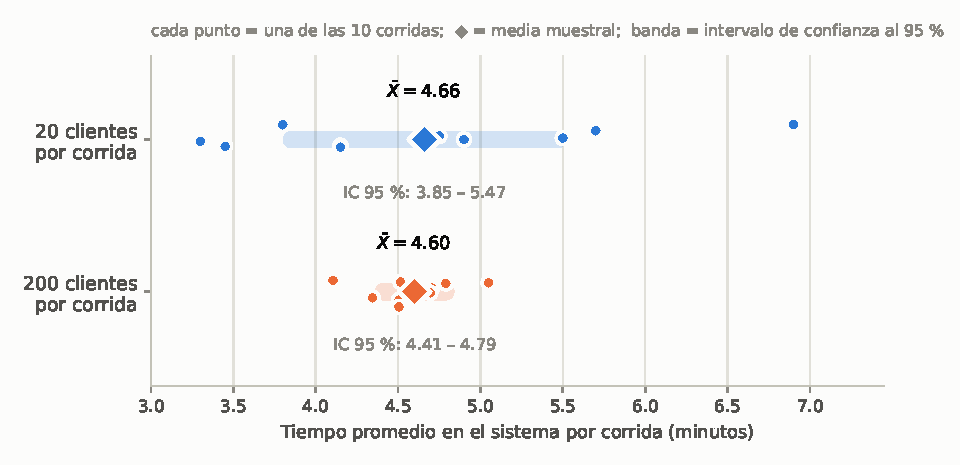
\includegraphics[width=0.95\textwidth]{fig_dispersion.pdf}
\caption{Tiempo promedio en el sistema obtenido en cada una de las diez corridas de cada escenario. Los dos conjuntos de puntos se centran prácticamente en el mismo lugar, pero el de 200 clientes está mucho más concentrado, lo que produce un intervalo de confianza notablemente más estrecho.}
\label{fig:dispersion}
\end{figure}

\subsection{Intervalos de confianza}

\begin{table}[H]
\centering
\caption{Intervalos de confianza al 95\,\% y 99\,\% de las medidas de desempe\~no ($n=10$ corridas de 200 clientes).}
\label{tab:ci200}
\footnotesize
\begin{tabular}{@{}lcrrrrrr@{}}
\toprule
Medida & Conf. & $\bar{X}$ & $S$ & $t_{n-1,1-\alpha/2}$ & $h$ & LI & LS \\
\midrule
Tiempo prom. en el sistema & 95\,\% & 4.6000 & 0.2642 & 2.2622 & 0.1890 & 4.4110 & 4.7890 \\
 & 99\,\% & 4.6000 & 0.2642 & 3.2498 & 0.2715 & 4.3285 & 4.8715 \\
\addlinespace
Porcentaje de tiempo ocioso & 95\,\% & 0.3607 & 0.0282 & 2.2622 & 0.0202 & 0.3405 & 0.3808 \\
 & 99\,\% & 0.3607 & 0.0282 & 3.2498 & 0.0290 & 0.3317 & 0.3896 \\
\addlinespace
Espera prom. por cliente & 95\,\% & 1.1115 & 0.2428 & 2.2622 & 0.1737 & 0.9378 & 1.2852 \\
 & 99\,\% & 1.1115 & 0.2428 & 3.2498 & 0.2495 & 0.8620 & 1.3610 \\
\addlinespace
Fracci\'on que esper\'o & 95\,\% & 0.3545 & 0.0539 & 2.2622 & 0.0385 & 0.3160 & 0.3930 \\
 & 99\,\% & 0.3545 & 0.0539 & 3.2498 & 0.0554 & 0.2991 & 0.4099 \\
\addlinespace
Espera prom. de quienes esperaron & 95\,\% & 3.1079 & 0.2972 & 2.2622 & 0.2126 & 2.8953 & 3.3205 \\
 & 99\,\% & 3.1079 & 0.2972 & 3.2498 & 0.3055 & 2.8024 & 3.4134 \\
\bottomrule
\end{tabular}
\begin{minipage}{\textwidth}\vspace{2pt}\footnotesize
LI y LS: l\'imites inferior y superior del intervalo. $t_{9,0.975}=2{,}2622$ y $t_{9,0.995}=3{,}2498$.
\end{minipage}
\end{table}

\paragraph{¿Qué se puede decir de la media y la desviación estándar muestral de cada medida?}

Las medias apenas se movieron respecto del escenario A, pero las desviaciones estándar cayeron en todas las medidas sin excepción. La del tiempo promedio en el sistema pasó de $1{,}1276$ a $0{,}2642$; la de la espera promedio por cliente, de $0{,}8430$ a $0{,}2428$; la del porcentaje ocioso, de $0{,}0910$ a $0{,}0282$. Son reducciones de entre el 62\,\% y el 77\,\%.

Hay un detalle que merece revisarse con calma. Si las medidas de cada corrida fueran promedios de observaciones independientes, multiplicar por diez la longitud de la corrida debería dividir la desviación estándar por $\sqrt{10} = 3{,}162$. Las razones $S_{20}/S_{200}$ que efectivamente se obtuvieron son 4,27 (tiempo en el sistema), 3,23 (tiempo ocioso), 3,47 (espera por cliente), 2,66 (fracción que esperó) y 3,49 (espera de quienes esperaron), todas agrupadas alrededor de ese 3,16 teórico. La coincidencia no es exacta, ni tenía por qué serlo: los tiempos de espera de clientes consecutivos están correlacionados entre sí, y diez corridas son pocas para estimar bien una desviación estándar. Aun así, confirma que el mecanismo que reduce la incertidumbre es el que se esperaba.

\paragraph{¿Qué análisis se puede hacer de los intervalos al 95\,\% y al 99\,\%?}

Los intervalos ahora sí resultan informativos. El del tiempo promedio en el sistema al 95\,\% va de 4,41 a 4,79 minutos: una amplitud de 0,38 minutos, apenas 23 segundos, contra los 1,61 minutos del escenario A. En términos relativos el margen bajó de $\pm 17{,}3\,\%$ a $\pm 4{,}1\,\%$. El del porcentaje de tiempo ocioso, entre 34,05\,\% y 38,08\,\%, contiene al valor teórico de 36,36\,\% y es lo bastante estrecho como para afirmar con seguridad que el cajero está desocupado alrededor de un tercio de la jornada.

Incluso la medida más problemática mejoró de manera sustancial: la espera promedio por cliente pasó de un margen de $\pm 51{,}3\,\%$ a uno de $\pm 15{,}6\,\%$. Sigue siendo la menos precisa de las cinco, lo cual es coherente, ya que es la que más depende de eventos poco frecuentes.

El paso del 95\,\% al 99\,\% conserva el mismo factor de 1,437 del escenario anterior, cosa que no podía ser de otro modo porque $n$ es igual en ambos casos. Pero ahora ese ensanchamiento se aplica sobre intervalos mucho más angostos y sale mucho más barato: el del tiempo en el sistema crece de 0,38 a 0,54 minutos y sigue siendo estrecho. Ahí está la ventaja práctica de trabajar con corridas largas: permite exigir un nivel de confianza alto sin sacrificar precisión útil.

% =====================================================
\section{Comparación de los dos escenarios}
% =====================================================

La Tabla~\ref{tab:resumen} confronta directamente las desviaciones estándar muestrales y los rangos de intervalo ($2h$) de los dos escenarios en los dos niveles de confianza.

\begin{table}[H]
\centering
\caption{Comparaci\'on de la desviaci\'on est\'andar muestral y del rango del intervalo de confianza ($2h$) entre los dos escenarios.}
\label{tab:resumen}
\footnotesize
\begin{tabular}{@{}lrrrrrr@{}}
\toprule
\multirow{2}{*}{Medida} & \multicolumn{2}{c}{$S$} & \multicolumn{2}{c}{Rango IC 95\,\% ($2h$)} & \multicolumn{2}{c}{Rango IC 99\,\% ($2h$)} \\
\cmidrule(lr){2-3}\cmidrule(lr){4-5}\cmidrule(l){6-7}
 & 20 cl. & 200 cl. & 20 cl. & 200 cl. & 20 cl. & 200 cl. \\
\midrule
Tiempo prom. en el sistema & 1.1276 & 0.2642 & 1.6133 & 0.3780 & 2.3177 & 0.5430 \\
Porcentaje de tiempo ocioso & 0.0910 & 0.0282 & 0.1302 & 0.0403 & 0.1870 & 0.0579 \\
Espera prom. por cliente & 0.8430 & 0.2428 & 1.2061 & 0.3474 & 1.7327 & 0.4990 \\
Fracci\'on que esper\'o & 0.1434 & 0.0539 & 0.2051 & 0.0771 & 0.2947 & 0.1107 \\
Espera prom. de quienes esperaron & 1.0386 & 0.2972 & 1.4860 & 0.4253 & 2.1348 & 0.6109 \\
\bottomrule
\end{tabular}
\end{table}

Comparar directamente las $S$ de las cinco medidas sería tramposo, porque están en unidades distintas (minutos unas, proporciones otras) y eso favorecería automáticamente a las que se miden en una escala más pequeña. La Tabla~\ref{tab:cv} corrige ese problema presentando la dispersión y la precisión en términos relativos, que son adimensionales y sí admiten comparación cruzada.

\begin{table}[H]
\centering
\caption{Precisi\'on relativa: coeficiente de variaci\'on ($S/\bar{X}$) y semiamplitud relativa al 95\,\% ($h/\bar{X}$), en porcentaje.}
\label{tab:cv}
\footnotesize
\begin{tabular}{@{}lrrrrr@{}}
\toprule
\multirow{2}{*}{Medida} & \multicolumn{2}{c}{$S/\bar{X}$ (\%)} & \multicolumn{2}{c}{$h/\bar{X}$ al 95\,\% (\%)} & \multirow{2}{*}{\makecell{Reducci\'on\\de $S$}} \\
\cmidrule(lr){2-3}\cmidrule(lr){4-5}
 & 20 cl. & 200 cl. & 20 cl. & 200 cl. & \\
\midrule
Tiempo prom. en el sistema & 24.20 & 5.74 & 17.31 & 4.11 & 76.6\,\% \\
Porcentaje de tiempo ocioso & 26.06 & 7.81 & 18.65 & 5.59 & 69.0\,\% \\
Espera prom. por cliente & 71.75 & 21.84 & 51.32 & 15.63 & 71.2\,\% \\
Fracci\'on que esper\'o & 40.96 & 15.20 & 29.30 & 10.87 & 62.4\,\% \\
Espera prom. de quienes esperaron & 33.41 & 9.56 & 23.90 & 6.84 & 71.4\,\% \\
\bottomrule
\end{tabular}
\end{table}

\begin{figure}[H]
\centering
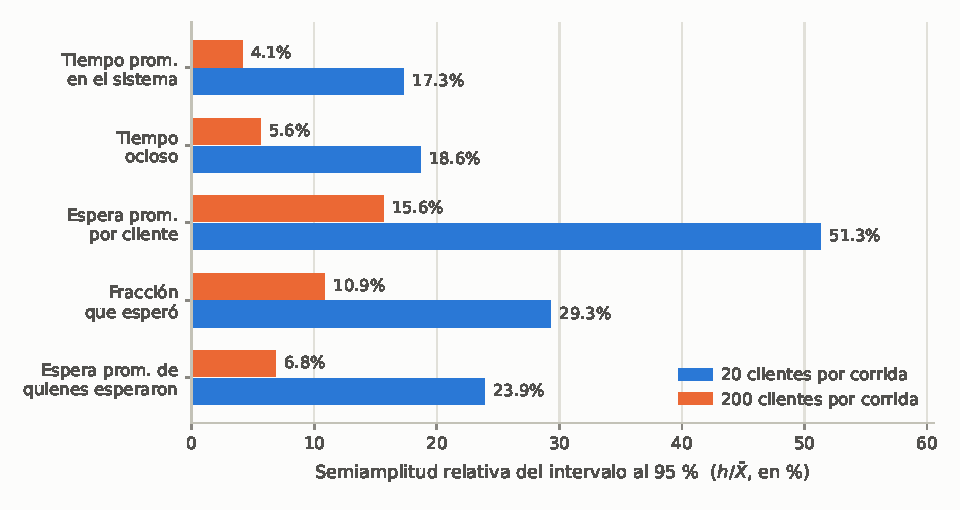
\includegraphics[width=0.95\textwidth]{fig_precision.pdf}
\caption{Semiamplitud relativa del intervalo de confianza al 95\,\% para cada medida de desempeño. Al pasar de 20 a 200 clientes por corrida, el margen de error se reduce a aproximadamente la tercera parte en las cinco medidas.}
\label{fig:precision}
\end{figure}

\subsection{¿Cuál combinación de número de clientes, repeticiones y porcentaje de confianza tiene la menor desviación estándar muestral y el menor rango de intervalo?}

Leyendo la Tabla~\ref{tab:resumen} en términos absolutos, la respuesta es la combinación de \textbf{200 clientes por corrida, 10 repeticiones y 95\,\% de confianza} aplicada al \textbf{porcentaje de tiempo ocioso}, que registra a la vez la menor desviación estándar muestral de toda la tabla ($S = 0{,}0282$) y el menor rango de intervalo ($2h = 0{,}0403$).

Esa lectura, sin embargo, hay que matizarla. Que el porcentaje de tiempo ocioso encabece la lista se debe en buena parte a que es una proporción acotada entre 0 y 1, mientras que las demás medidas se expresan en minutos y toman valores del orden de la unidad o mayores. Al mirar la Tabla~\ref{tab:cv}, que elimina el efecto de las unidades, la medida más precisa en términos relativos resulta ser el tiempo promedio en el sistema, con un margen de apenas $\pm 4{,}1\,\%$ frente al $\pm 5{,}6\,\%$ del tiempo ocioso.

Lo que sí es robusto, y se cumple con cualquiera de los dos criterios, es la conclusión sobre los factores que están en juego:

\begin{enumerate}[itemsep=3pt]
    \item \textbf{La longitud de la corrida es el factor dominante.} Para las cinco medidas, sin excepción, 200 clientes producen menor $S$ y menor rango que 20 clientes. La mejora oscila entre el 62\,\% y el 77\,\% y no depende del nivel de confianza elegido.
    \item \textbf{El nivel de confianza actúa como un multiplicador fijo.} Con $n = 10$ corridas, pasar del 95\,\% al 99\,\% ensancha todo intervalo en un factor de 1,437, siempre. No altera $S$, que es una propiedad de los datos y no de la decisión estadística.
    \item \textbf{El número de repeticiones no se varió, pero su efecto es predecible.} La fórmula $h = t\,S/\sqrt{n}$ indica que reducir $h$ a la mitad manteniendo la corrida corta exigiría cuadruplicar $n$, es decir, pasar de 10 a 40 corridas. En este experimento resultó más económico alargar las corridas que multiplicarlas.
\end{enumerate}

La combinación óptima, entonces, es \textbf{corridas largas con el menor nivel de confianza que resulte aceptable} para la decisión que se quiera tomar. Y aquí va una advertencia: el intervalo más estrecho no es automáticamente el mejor. Un intervalo del 95\,\% es más angosto que uno del 99\,\% simplemente porque acepta equivocarse una de cada veinte veces en lugar de una de cada cien. La estrechez solo es una virtud cuando viene de reducir la variabilidad, como al pasar de 20 a 200 clientes, y no cuando viene de rebajar la exigencia de confianza.

% =====================================================
\section{Conclusiones}
% =====================================================

\begin{enumerate}[itemsep=4pt]
    \item La simulación \emph{ad hoc} de un sistema de cola simple reproduce, con aritmética elemental y dos variables aleatorias uniformes discretas, el comportamiento esencial de un sistema de espera real. Las seis recurrencias del modelo bastan para generar las nueve columnas de la tabla y, a partir de ellas, las cinco medidas de desempeño.

    \item Los resultados de una única corrida no permiten caracterizar el sistema. En el escenario de 20 clientes, corridas ejecutadas bajo condiciones idénticas arrojaron tiempos promedio en el sistema que iban de 3,30 a 6,90 minutos. Presentar cualquiera de ellas como \guillemotleft el resultado\guillemotright{} habría sido tan defendible como arbitrario.

    \item Alargar la corrida de 20 a 200 clientes no modificó las medias estimadas (4,66 frente a 4,60 minutos en el sistema) pero sí redujo las desviaciones estándar muestrales entre un 62\,\% y un 77\,\%. Las razones de reducción observadas se agruparon en torno al valor $\sqrt{10} = 3{,}162$ que predice la teoría, lo que confirma que la ganancia de precisión proviene de promediar más observaciones y no de un cambio en el sistema simulado.

    \item Los intervalos de confianza cuantifican esa ganancia de manera directa. El margen relativo del tiempo promedio en el sistema pasó de $\pm 17{,}3\,\%$ con 20 clientes a $\pm 4{,}1\,\%$ con 200, y el de la espera promedio por cliente, la medida más ruidosa de las cinco, de $\pm 51{,}3\,\%$ a $\pm 15{,}6\,\%$.

    \item El nivel de confianza no aporta información nueva, solo redistribuye el compromiso entre certeza y precisión: con diez repeticiones, exigir 99\,\% en lugar de 95\,\% ensancha todo intervalo en un factor constante de 1,437.

    \item La simulación reprodujo los valores teóricos del modelo. El porcentaje de tiempo ocioso promedio con 200 clientes fue de 36,07\,\%, frente al 36,36\,\% que predice la utilización $\rho = E[S]/E[A]$, y el intervalo al 95\,\% de esa medida contiene el valor teórico. Esta coincidencia funciona como validación independiente de todo el procedimiento.

    \item Desde el punto de vista práctico, el sistema simulado está sobredimensionado: el cajero permanece desocupado cerca de un tercio de su jornada mientras que solo el 35\,\% de los clientes espera, y en promedio poco más de tres minutos. Sin embargo, la sola comparación de las dos medidas de espera revela que el costo de la congestión no se distribuye de manera uniforme, sino que recae concentrado sobre una minoría de usuarios. Una decisión gerencial basada únicamente en el promedio general subestimaría el problema.
\end{enumerate}

% =====================================================
\section{Anexos}
% =====================================================

Se adjuntan a este informe los archivos con los datos registrados y ejecutados:

\begin{itemize}[itemsep=3pt]
    \item \texttt{fila\_banco\_20\_clientes.xlsx} --- hoja \guillemotleft Ejemplo\guillemotright{} con la tabla completa de la simulación de 20 clientes y las medidas de desempeño calculadas mediante fórmulas, y hoja \guillemotleft 10 runs\guillemotright{} con los resultados de las diez corridas, su media, su desviación estándar y los intervalos de confianza.
    \item \texttt{fila\_banco\_200\_clientes.xlsx} --- misma estructura, para el escenario de 200 clientes.
    \item \texttt{Confidence\_intervals\_20\_200.ipynb} --- cuaderno de Google Colab, adaptado del cuaderno \texttt{Confidence intervals.ipynb} suministrado en la guía. Contiene el motor de simulación, la verificación contra la Tabla 1.1 de \cite{Banks1998}, la generación de las corridas de ambos escenarios y el cálculo de los intervalos de confianza al 95\,\% y 99\,\% presentado con el mismo formato del Ejemplo 2 de la subsección 1.11.1. El cuaderno se entrega ya ejecutado y, gracias a la semilla fija, reproduce exactamente las tablas de este informe.
\end{itemize}

% =====================================================
\begin{thebibliography}{9}
\bibitem{Banks1998}
Banks, J. (1998). \emph{Handbook of Simulation: Principles, Methodology, Advances, Applications, and Practice}. John Wiley \& Sons, Inc. Capítulo 1.
\end{thebibliography}

\end{document}
